\documentclass{article}
\usepackage[utf8]{inputenc}

\title{Optimization of Spatial Architectures for\\Acceleration of Machine Learning}
\author{Mateja Putic}
\date{Spring 2018}

\usepackage{palatino}
\usepackage{natbib}
\usepackage{graphicx}
\usepackage{booktabs} % For formal tables
\usepackage[letterpaper, margin=1in]{geometry}
\usepackage{caption}
\usepackage{subcaption}
\usepackage{xspace}
\usepackage{xfrac}

\newcommand\paragraphHeading[1]{\textbf{#1:}\xspace}
\newcommand\eg{\emph{e.g.}\xspace}
\newcommand\ie{\emph{i.e.}\xspace}
\newcommand\etc{\emph{etc.}\xspace}
\newcommand\viz{\emph{viz.}\xspace}
\newcommand{\oneSub}[2]{$\textrm{#1}_{#2}$}
\newcommand{\twoSub}[3]{$\textrm{#1}_{#2,#3}$}
\newcommand\dyhardDnn{DyHard-DNN\xspace}
\newcommand\dyhardDnns{{\dyhardDnn}s\xspace}
\newcommand\dyhardXplore{DyHard-Xplore\xspace}
\newcommand\bpc{\ensuremath{~\sfrac{\textrm{Bytes}}{\textrm{Cycle}}}}

\newcommand\Nin{\ensuremath{N_\textrm{in}}}
\newcommand\Nout{\ensuremath{N_\textrm{out}}}
\newcommand\Nij{\ensuremath{N_{ij}}}
\newcommand\Ni{\ensuremath{N_i}}
\newcommand\Nj{\ensuremath{N_j}}
\newcommand\Nki{\ensuremath{K_{i}}}
\newcommand\Nkj{\ensuremath{K_{j}}}
\newcommand\Kij{\ensuremath{K_{ij}}}
\newcommand\Nkij{\ensuremath{K_{ij}}}

\newcommand\googlenet{GoogLeNet\xspace}
% Set line spacing
% \renewcommand{\baselinestretch}{1.15}

\begin{document}

\maketitle

\section{Introduction}

\textbf{Machine Learning Automates Extraction of Meaning From Big Data}
While the age of big data has enabled efficient large-scale data collection, automated analysis remains essential for extracting high semantic meaning quickly and on a large scale.
Machine learning has offered a compelling set of solutions to this application domain because of its ability to autonomously identify structure and correlations in large datasets~\cite{economist2010data}.
DNNs have successfully been deployed in platforms ranging from cloud services to embedded devices in image recognition and classification, cancer diagnosis, spam filtering, voice recognition, and applications controlling self-driving vehicles ~\cite{hannun2014deep, he2016deep, hinton2012deep, krizhevsky2012imagenet, li2016persona, silver2016mastering, jafari2016extraction, fridman2017autonomous}.

\textbf{Machine Learning Creates Massive Computation Demands}
Due to the implementation details of state-of-the-art DNNs, these algorithms are very computationally expensive.
Tera- or peta-byte sized training sets are required for high accuracy, many arithmetic operations are required for a single inference, models can have up to 100 layers, and many parallel inference requests require running the model many times or continuously~\cite{dean2017nips}.
While demand for DNN performance has largely benefited from the relatively recent introduction of large GPUs that offer parallel computational capability~\cite{parloff2016why}, concerns about power and reliability~\cite{snir2014addressing} have grown proportionally, across deployment scales.

\textbf{Machine Learning Algorithms Map Well to Spatial Architectures} 
Machine learning algorithms are often realized as a directed graph of compute operations with varying degrees of data sharing between nodes.
Spatial architectures are a class of hardware architecture that are characterized by a large array of identical compute units, a shared memory architecture, and an interconnect network that allows them to communicate~\cite{parashar2013triggered, kung1982wavefront, kung1984supercomputing}.
Spatial architectures are a good fit for machine learning algorithms because they can exploit varying degrees of data reuse across multiple dimensions of their inputs to capture abundantly available thread parallelism in DNN dataflows.
Examples of classical spatial architectures with such characteristics are TRIPS~\cite{sankaralingam2003exploiting}, Raw~\cite{taylor2002raw}, Imagine~\cite{keckler2009multicore}, and more recently, Google's Tensor Processing Unit~\cite{jouppi2017datacenter}, Graphcore~\cite{knowles2017designing}, and the Micron Automata Processor~\cite{dlugosch2014efficient}, as well as embedded platforms like Minerva~\cite{reagen2016minerva}, Eyeriss~\cite{chen2016eyeriss}, ShiDianNao~\cite{du2015shidiannao}, and EIE~\cite{han2016eie}.
Further optimization of hardware metrics of spatial architectures warrants understanding major properties of these algorithms.

\textbf{Machine Learning Algorithms Have Diverse Workload Characteristics}
There exist a large number of DNN networks used for various applications, each of which are comprised of a sequence of operational layers.
Within networks, there exists intra-network diversity among layers of differing types, \eg, convolution, activation, and pooling, \etc.
Although a majority of the operations in DNNs are implemented by GEMM, the data structures between these layers have varying dimensions, \ie, shape and rank.
% While inter-network diversity in DNN models is well known, there also exists intra-network diversity, \viz, among layers of differing types (\eg, convolution, activation, pooling, \etc), and among layers of the same type (\eg,  input, output dimensions, \etc)~\cite{chakradhar2010dynamically, venkataramani2014axnn}.
As a consequence of this diversity, DNN program phases present a wide range of operational intensities to the underlying hardware, resulting in varied utilization in a fixed hardware architecture.
% The key idea of achieving exploiting these characteristics with this type of architecture is to identify data and task parallelism available in the algorithms, and spatial and temporal locality within the data, and to distribute work among a large number of parallel resources and reusing data whenever possible.

\textbf{Machine Learning Algorithms Have Flexible Semantics}
DNNs have an abundance of resilience properties that can be leveraged to design more efficient spatial architecture DNN accelerators.
The functionality and accuracy of DNNs has been shown to be resilient to distortion and noise in inputs by \textit{generalization} of exact functions achieved through training~\cite{cheng2017maximum, dodge2017quality, szegedy2013intriguiing, zhou2017classification}.
To avoid overfitting toward improving function generalization and achieving high accuracy, modern DNN training includes \textit{pruning} the least important parameters, as determined by backpropagation of error~\cite{molchanov2016pruning, srivastava2014dropout, han2015learning}.
Additionally, DNNs are resilient to changes in network architecture, for example, by replacement of layers by operations with reduced data requirements and lower operational intensity~\cite{lin2013network, szegedy2015going}.
Several parameter approximation and quantization methods for DNNs have been applied to save memory and compute cycles to improve their performance, and make them suitable for deployment on memory-constrained platforms~\cite{vanhoucke2011improving, denton2014exploiting, gong2014compressing}.
Furthermore, several previous works have demonstrated that resilience properties of neural networks can be leveraged to improve runtime hardware characteristics~\cite{du2014leveraging, venkataramani2013quality, yu2017scalpel}

\section{Problem Definitions and Research Hypothesis}

Broadly, the challenge to be addressed by this work is to develop methodologies for the design of spatial architectures to accelerate a broad class of DNN applications and to give hardware designers tools to explore tradeoff spaces between application and hardware metrics. 
We do this by recognizing that if algorithmic properties of DNNs are heterogeneous in nature, then they can be exploited to make changes at the hardware level to improve and make tradeoffs and improve resource usage.
To approach this challenge systematically, we identify three specific research problems to be addressed:

\textbf{Problem 1: Statically Allocated DNN Accelerator Hardware Present Unclaimed Design Margins} Inter- and intra-network diversity in DNN workloads result in diversity in the utilization of hardware throughout the execution phases of a DNN network.
As a consequence, statically allocated accelerator hardware runs sub-optimally and leaves energy-efficiency margins unclaimed, creating opportunities for optimization of runtime metrics based on prior knowledge of these characteristics.
To give hardware designers a tool to better align application requirements with resources available in the deployment scenario, what is needed is a methodology to design hardware that takes advantage of the workload diversity to make DNN execution more efficient, and to enable tradeoffs between better performance and lower power.

\textbf{Problem 2: Biological Neuron Algorithms Lack Performance and Scalability on von Neumann Architectures} Capturing a large degree of parallelism available in machine learning algorithms in hardware is challenging for two reasons: (i) existing hardware may have a small number of cores, bounding the maximum degree of parallelism, and (ii) memory access patterns within dataflow graphs exhaust traditional von Neumann memory hierarchy.
Both of these issues limit scalability on such architectures, consequently limiting their throughput and performance.
To demonstrate how to capture a large degree of parallelism and to make use of the scalability advantages of spatial architectures, what is needed is a demonstration of the process of developing a mapping of biological neurons to a spatial architecture, and the evaluation of the performance and resource scalability.

\textbf{Problem 3: Soft Error Protection Techniques Designed Without Application Knowledge Present Unclaimed Design Margins} Existing methods for soft error protection do not consider the application-level characteristics, and apply protection techniques uniformly.
Consequently, a significant design margin exists for operations that are inherently resilient, and do not need the additional hardware-level protection.
To give hardware designers a tool for improving DNN accelerator reliability, what is needed is a methodology to for identifying opportunities to leverage DNN resilience to reclaim design margins in the implementation of soft error protection techniques, and to make tradeoffs between reliability, power and performance.

% The result of this work will be a set of tools that assist in the characterization of the impacts of those tradeoffs and for optimization of hardware characteristics based on prior knowledge of DNN algorithm workloads.

\noindent\\
To address the identified problems, we propose three tasks that will study performance, scalability, power, and resilience optimizations of machine learning workloads on spatial architectures.

\textbf{Task 1: Leverage Dynamic Workload Characteristics to Optimize Hardware Efficiency of Spatial Architectures}
To make the case for dynamically configurable DNN hardware, in this task, we will study the workload characteristics of several DNN workloads.
To address the challenge of low power DNN acceleration, and to give hardware designers tools to make tradeoffs between power and performance in DNN accelerator design, we will introduce a reconfigurable hardware paradigm, and will develop a methodology for systematic exploration of the design space. 
We propose a methodology for the design of reconfigurable DNN hardware that determines the best configuration for each DNN layer, while considering reconfiguration cost, across costs that consider both ASIC and FPGA platforms to improve latency and energy efficiency.
    
\textbf{Task 2: Exploit Resilience to Accelerate Biological Neurons on a Spatial Architecture}
This task will study the correspondences between Hierarchical Temporal Memory and the cell-like spatial computing fabric of the Automata Processor.
To address the memory bottleneck problem in traditional memory hierarchies, we will propose a methodology for realization of Hierarchical Temporal Memory as automata.
We will identify correspondences between these two computing paradigms, develop an efficient mapping, and evaluate performance and resource scalability.
The result of this work will be a tool that will allow HTM application designers to synthesize, simulate, and validate performance of HTM applications with the Automata Processor.

\textbf{Task 3: Exploit Resilience to Optimize Hardware Efficiency of Resilient Spatial Architectures}
To address the challenge of optimizing the performance and power metrics in resilient DNN accelerators, in this task we will develop methods for optimization of soft error protection techniques based on the criticality of neurons in a DNN.
We will develop methods for sensitivity characterization, applying selective soft error protection based on a classification of neuron sensitivity, and simultaneous optimization of application accuracy and hardware resources.
The result of this work will be a tool for making tradeoffs between resilience, power, and performance in the presence of faults to give hardware designers a tool for the design of efficient, resilient DNN accelerators.

\noindent\\
The remainder of this proposal is organized as follows. 
Sections 3, 4, and 5 introduce the three areas of research as part of this program.
Each of these sections contains four subsections.
Subsection 1 provides a problem definition. 
Subsection 2 a research hypothesis.
Subsection 3 highlights major contributions.
Subsection 4 provides further motivation of the problem. 
Subsection 5 introduces the proposed approach, and highlights preliminary results that justify the insights and provide risk minimization for the overall project.
Subsection 6 states evaluation criteria to determine success in the project.
In Subsection 7, we present an analysis of related work, and differentiate our approach from previous approaches the defined challenges.
Finally, in the Appendix, we document a summary and plan of work that details completed work and work left to be done.

\section{Task 1: Hardware Optimization Based On Workload Characteristics} 

\subsection{Problem Definition}

Existing custom DNN hardware accelerators encompassing low-power ASICs~\cite{reagen2016minerva,chen2017eyeriss,du2015shidiannao}, FPGAs~\cite{chung2017accelerating}, and large-scale accelerator systems~\cite{venkataramani2017scaledeep, chen2014dadiannao,jouppi2017datacenter} are specialized to leverage the fine-grained data parallelism, dataflow structure, and communication patterns in DNNs to achieve substantially better energy--efficiency over CPUs and GPUs.
DNNs exhibit significant heterogeneity in their computational characteristics, \ie, feature and kernel dimensions, and dramatic variances in computational intensity, even between adjacent layers in one DNN.
However, a key limitation of these architectures is that their microarchitectural parameters are \emph{statically} determined at design time, and consequently, they run sub-optimally and leave energy--efficiency margins unclaimed.

The key idea of the proposed approach is to reconfigure the microarchitectural parameters of the accelerator dynamically, based on the characteristics of the layer under execution.
Consequently, performance and energy benefits can be achieved beyond statically configured accelerators with different reconfiguration overheads taken into account.
The costs of augmenting the accelerator with the ability to reconfigure depends on the implementation scenario.
For example, in the case of ASIC designs, under an iso-power constraint, reconfiguration involves clock/power-gating computation slices or interconnect links based on DNN layer dimensions.
In contrast, reconfiguration in FPGA designs involves loading a new full or partial bitstream.

The insight enabling this idea is that layer dimensions are known before execution begins, so the best configuration for each layer can be determined offline.
To this end, we will develop a methodology that in the \emph{offline phase}, takes in a description of the DNN layers, the microarchitectural parameters of an accelerator augmented with \emph{run time control logic}, a performance model that quantifies its run time, and the costs of reconfiguration.
It explores the space of possible configurations to construct a \emph{configuration map} with the best per-layer configurations, while minimizing the metric of interest, despite overhead cost.
Then in the \emph{execution phase}, configuration logic will enforce the configuration map to dynamically improve latency and energy--efficiency.

\subsection{Research Hypothesis}
In proposing this work, we hypothesize that \textit{if} DNN accelerator hardware is dynamically reconfigured according to the workload characteristics of each layer, \textit{then} a configuration map will be found that allows the accelerator to execute the workload with better runtime characteristics than under a static conditions.

\subsection{Contributions}
This research will make the following contributions:

\begin{itemize}
    \item To improve the energy-efficiency of DNN accelerators, we will develop a new approach for dynamically configuring accelerator microarchitectural parameters that exploits the diversity in the computational characteristics of DNN layers.
    \item We will describe a DNN accelerator optimization methodology, consisting of: (i) an \emph{offline} phase, wherein the configuration map to execute each layer is identified, considering costs of reconfiguration, and (ii) a \emph{run time} phase, wherein the configuration map is enforced as the DNN layers execute on the accelerator 
    \item To identify optimization opportunities for accelerator designers, we will study the latency--energy trade-off space by dynamic reconfiguration of microarchitectural parameters, across a range of overhead costs modeling ASIC and FPGA platforms. 
\end{itemize}

The proposed methodology will be evaluated in the context of a SIMD 2D systolic array architecture with an on-chip scratchpad memory, synthesized to a commercial 14~nm low power technology~\cite{venkataramani2017scaledeep}.

\subsection{Motivating Dynamic Spatial Array Hardware}

In this section, we motivate the need for dynamic reconfiguration by analyzing a popular DNN benchmark and identify opportunities for improving performance and efficiency.

\begin{table}
  \caption{VGG11 Parameters and Characteristics}
  \label{tbl:vgg_params}
  \centering
  \footnotesize
  \setlength\tabcolsep{4pt}
  \begin{tabular}{lrrccrrr}
    \toprule 
     & \multicolumn{4}{c}{Parameters} & \multicolumn{3}{c}{Compute Characteristic} \\
     \cmidrule(rl){2-5} \cmidrule(rl){6-8}
     Layer & $\Nin$ & $\Nout$ & $\Nij$ & $\Kij$ & Ops (M) & Bytes (M) & $\sfrac{\textrm{Ops}}{\textrm{Byte}}$ \\
    \midrule
    \oneSub{CONV}{1} & 3 & 64 & $224\times224$ & $3\times3$ & 173.41 & 6.73 & 25.78 \\
    \oneSub{CONV}{2} & 64 & 128 & $112\times112$ & $3\times3$ & 1849.69 & 4.96 & 372.59 \\
    \twoSub{CONV}{3}{1} & 128 & 256 & $56\times56$ & $3\times3$ & 1849.69 & 3.00 & 616.92 \\
    \twoSub{CONV}{3}{2} & 256 & 256 & $56\times56$ & $3\times3$ & 3699.38 & 4.39 & 842.51 \\
    \twoSub{CONV}{4}{1} & 256 & 512 & $28\times28$ & $3\times3$ & 1849.69 & 3.56 & 519.06 \\
    \twoSub{CONV}{4}{2} & 512 & 512 & $28\times28$ & $3\times3$ & 3699.38 & 6.32 & 584.95 \\
    \twoSub{CONV}{5}{1} & 512 & 512 & $14\times14$ & $3\times3$ & 924.84 & 5.12 & 180.63 \\
    \twoSub{CONV}{5}{2} & 512 & 512 & $14\times14$ & $3\times3$ & 924.84 & 5.12 & 180.63 \\
    \oneSub{FC}{6} & 25088 & 4096 & $1\times1$ & $1\times1$ & 205.52 & 205.58 & 1.00 \\
    \oneSub{FC}{7} & 4096 & 4096 & $1\times1$ & $1\times1$ & 33.55 & 33.57 & 1.00 \\
    \oneSub{FC}{8} & 4096 & 1000 & $1\times1$ & $1\times1$ & 8.19 & 8.20 & 1.00 \\
    \bottomrule 
  \end{tabular}
%%  \includegraphics[width=\columnwidth]{fig/vgg-ops.pdf}
\end{table}

\subsubsection{Diversity in DNN Workloads}

To further motivate the proposed approach, Table~\ref{tbl:vgg_params} shows the dimensions and compute characteristics of each layer in the VGG11 image classification DNN~\cite{simonyan2014very}.
VGG11 contains eight CONV and three FC layers.
Although each layer performs the same type of operation, either 2D-convolution or matrix-vector multiplication, \emph{data-structure shape and Ops/Byte requirements vary dramatically}.

We observe from Table~\ref{tbl:vgg_params} that the initial CONV layers are shallow and stout, \ie, they have very few input and output features ($\Nin$ and $\Nout$), but the feature dimensions ($\Nij$) are quite large.
As we progress to the final layers, $\Nin$ and $\Nout$ increase by over two orders of magnitude, while $\Nij$ decreases proportionately.
In the case of more recent DNNs, \eg, GoogLeNet~\cite{szegedy2015going} and ResNet~\cite{he2016deep}, even $\Kij$ varies more frequently, between $7\times7$ to $1\times1$.
The dimensions directly impact the OPs/Byte of each layer.
The CONV layers are dominated by sizes of the input and output volumes, while FC layers are dominated by weights.
Also, CONV layers offer abundant opportunities for data-reuse, while FC layers are limited by memory bandwidth.
We find the OPs/Byte requirement to vary by over an order of magnitude even within the CONV layers, and by over two orders of magnitude overall.

\subsubsection{Limits of Statically Configured Hardware}

Workload diversity translates to a loss of utilization at design-time in statically configured accelerators due to two main factors.

\textbf{Ops-to-byte ratio}
DNN accelerator designers allocate resources for compute, memory and interconnect such that performance is optimal for common layers.
When the layer has abundant data-reuse, (\eg, CONV layers with $\textrm{Ops}/\textrm{Byte}_\textrm{layer} > \textrm{Ops}/\textrm{Byte}_\textrm{hw}$), the accelerator is under-provisioned in compute, \ie, resources could be shifted from memory bandwidth to compute, by powering up/down execution engines and interconnect channels.
In contrast, layers with poor data-reuse (\eg, FC layers $\textrm{Ops}/\textrm{Byte}_\textrm{layer} < \textrm{Ops}/\textrm{Byte}_\textrm{hw}$) underutilize compute, as they are unable feed data to the processing elements at a sufficient rate.
Both scenarios result in unclaimed performance and energy margins.

\textbf{Residual effects} 
The main computational work in DNN accelerators is done by a multi-dimensional array of compute elements.
If a hardware dimension is not an even multiple of the workload dimension, it results in a utilization drop.
Imbalanced work divisions along each dimension have a multiplicative effect, and the performance drop builds up very quickly.

\subsubsection{Reconfigurable SIMD Systolic Arrays} 
\label{sec:syst-array}

We illustrate the benefits of dynamic reconfiguration using a generic SIMD 2D systolic array architecture common in DNN hardware literature~\cite{venkataramani2017scaledeep,chen2017eyeriss,chen2014dadiannao}, such as shown in Figure~\ref{fig:systolic_array}. 
Specifically, we consider the embodiment proposed in ScaleDeep~\cite{venkataramani2017scaledeep}, wherein the architecture is comprised of a 2D array of processing elements (PE), with each PE connected to its neighbors.
The PEs are a SIMD array of multiply-accumulate units.
The number of rows ($R$), columns ($C$) and SIMD lanes ($L$) define the compute capability of the architecture.
The accelerator also contains three scratchpad memories, one each to store the input, weight and output data structures.
The capacities and bandwidth with which the PE array is interfaced to the input, weight, and output memories are given by $\textrm{Cap}_\textrm{IM}$, $\textrm{Cap}_\textrm{WM}$ and $\textrm{Cap}_\textrm{OM}$, and $\textrm{BW}_\textrm{IM}$, $\textrm{BW}_\textrm{WM}$ and $\textrm{BW}_\textrm{OM}$, respectively.
Within the scope of this work, we enable run time reconfiguration of the compute array dimensions, memory capacity and interconnect bandwidth.

% To realize convolution and matrix-vector multiplication, we adopt an output stationary dataflow.
% In this case, the input is fed along the rows, and the weights are fed along the columns.
% The partial sums are accumulated within the PEs, and are further accumulated diagonally before being stored in the output memory.
% Specifically, the $\Nij$, $\Kij$ and $\Nout$ workload dimensions are mapped spatially to the rows ($R$), columns ($C$) and SIMD lanes ($L$) of the PE array, while the $\Nin$ dimension is sequenced temporally.

\begin{figure*}
    \centering
    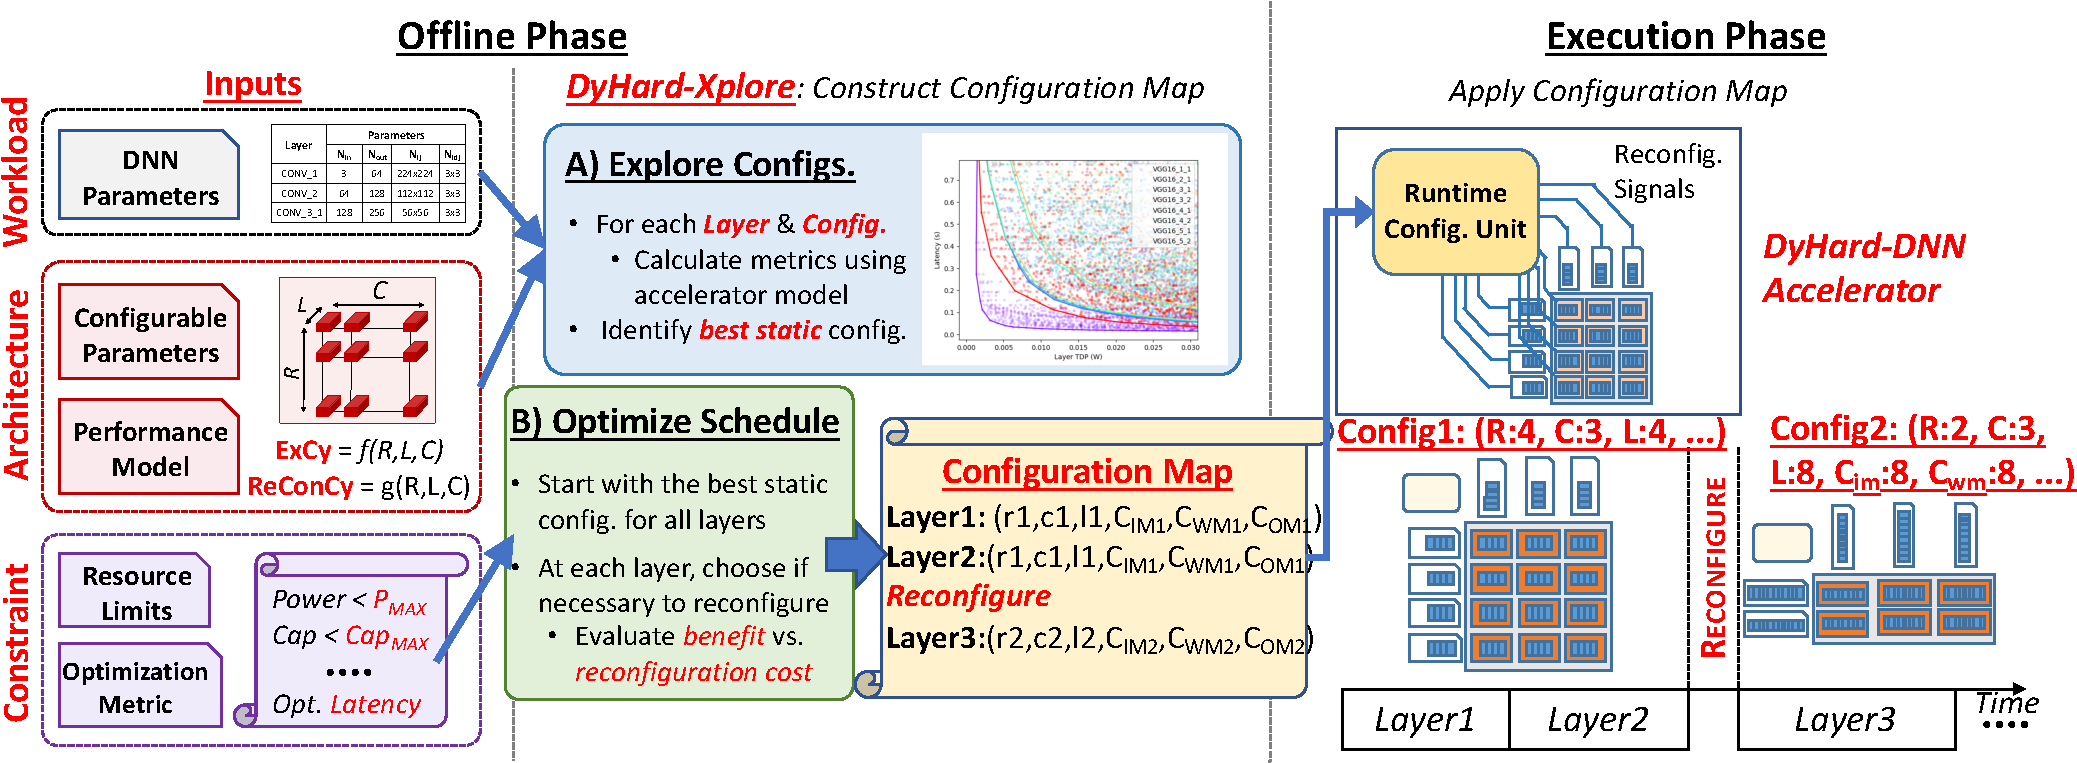
\includegraphics[width=\linewidth]{figs/dyHard-dnn-overview.pdf}
    \caption{Overview of DyHard-DNN methodology}
    \label{fig:overview}
\end{figure*}

\subsection{Proposed Approach}

Figure~\ref{fig:overview} shows an overview of the proposed approach encompassing \emph{offline analysis} and \emph{run-time execution} phases. 
An analysis tool will determine optimal microarchitectural parameters on a layer-by-layer basis and will construct an optimized \emph{configuration map} that specifies per-layer run-time configurations, incorporating inter-layer reconfiguration cost.
During execution, free microarchitectural parameters will be bound to values specified by the configuration map.

Within this study, we will develop the following components:
\begin{itemize}
\item \textbf{Reconfigurable SIMD Systolic Array Architecture}
The reconfigurable systolic array platform will define and identify the bounds of reconfigurable parameters, \eg, rows, columns, SIMD lanes, \etc,  that will be available to the optimization methodology.
\item \textbf{Optimization Methodology}
The optimization methodology will consist of an offline phase, in which a configuration map is constructed for each hardware design candidate.
In the runtime phase, the methodology will dictate how the systolic array will be reconfigured to meet the target metrics of interest.
\item \textbf{Optimization Tool} 
The optimization tool will construct a configuration map from the dimensional parameters of a DNN layer.
These will be used to generate a sequence of configurations while considering total physical design constraints and the cost of reconfiguration on a given circuit substrate.
This tool will also facilitate evaluation of the performance and power of a given schedule of execution on the proposed reconfigurable systolic array architecture.
\end{itemize}

\subsection{Evaluation Criteria}

We will demonstrate dynamic reconfiguration in the context of the 2D systolic array architecture using simulation.
We will consider two concrete scenarios where \dyhardDnns could be deployed: (i) an embedded ASIC implementation and (ii) programmable SoCs with embedded FPGAs, \eg, Intel Harp or Xilinx Zync. 
Success in this project will be achieved if simulation shows that dynamic configurations achieve better performance or power options than static when taking into account the costs of reconfiguration.
% Impact will be facilitated by publication of the research findings and release of the optimzation tool and associated documentation as open source software.

% We will construct the configuration map from the following inputs:
% \begin{enumerate}
%     \item \textbf{DNN Workload:} The parameters \{$\Nin$, $\Nout$, $\Nij$, $\Kij$\} describing the computations in DNN layer
%     \item \textbf{Accelerator Architecture:} A description of the DNN accelerator (specifying configurable microarchitectural parameters), a performance model, and the cost of reconfiguration
%     \item \textbf{Constraints:} A list of resource constraints (\eg, a limit on the total power consumed, on-chip memory capacity, \etc) that each configuration should meet and a metric-of-interest for optimization, \eg, performance or energy
% \end{enumerate}

% \paragraphHeading{Offline Phase}
% For the offline phase, we develop a methodology, \emph{DyHard-Xplore}, which is comprised of two key steps.
% First (i), for each layer, based on the workload dimensions and dataflow, we identify the valid range for each microarchitectural parameter and enumerate the design space of configurations.
% We also identify the best static configuration to execute all layers, if dynamic reconfiguration were prohibited.
% Then (ii), starting with the static configuration as an initial configuration for all layers, we iteratively improve the global metric of interest by choosing among staying at the best configuration for the previous layer, or switching to the current layer's best choice and paying the cost of reconfiguration.
% We elaborate on the \dyhardXplore algorithm in Section~\ref{sec:dyhard-xplore}.

% \paragraphHeading{Execution Phase}
% The layer configuration map from the offline phase is pre-loaded prior to execution onto the accelerator's run time configuration unit (RCU).
% As DNN layers execute on the accelerator, the RCU interrupts and reconfigures the accelerator, as specified in the configuration map.

\begin{figure}
    \centering
    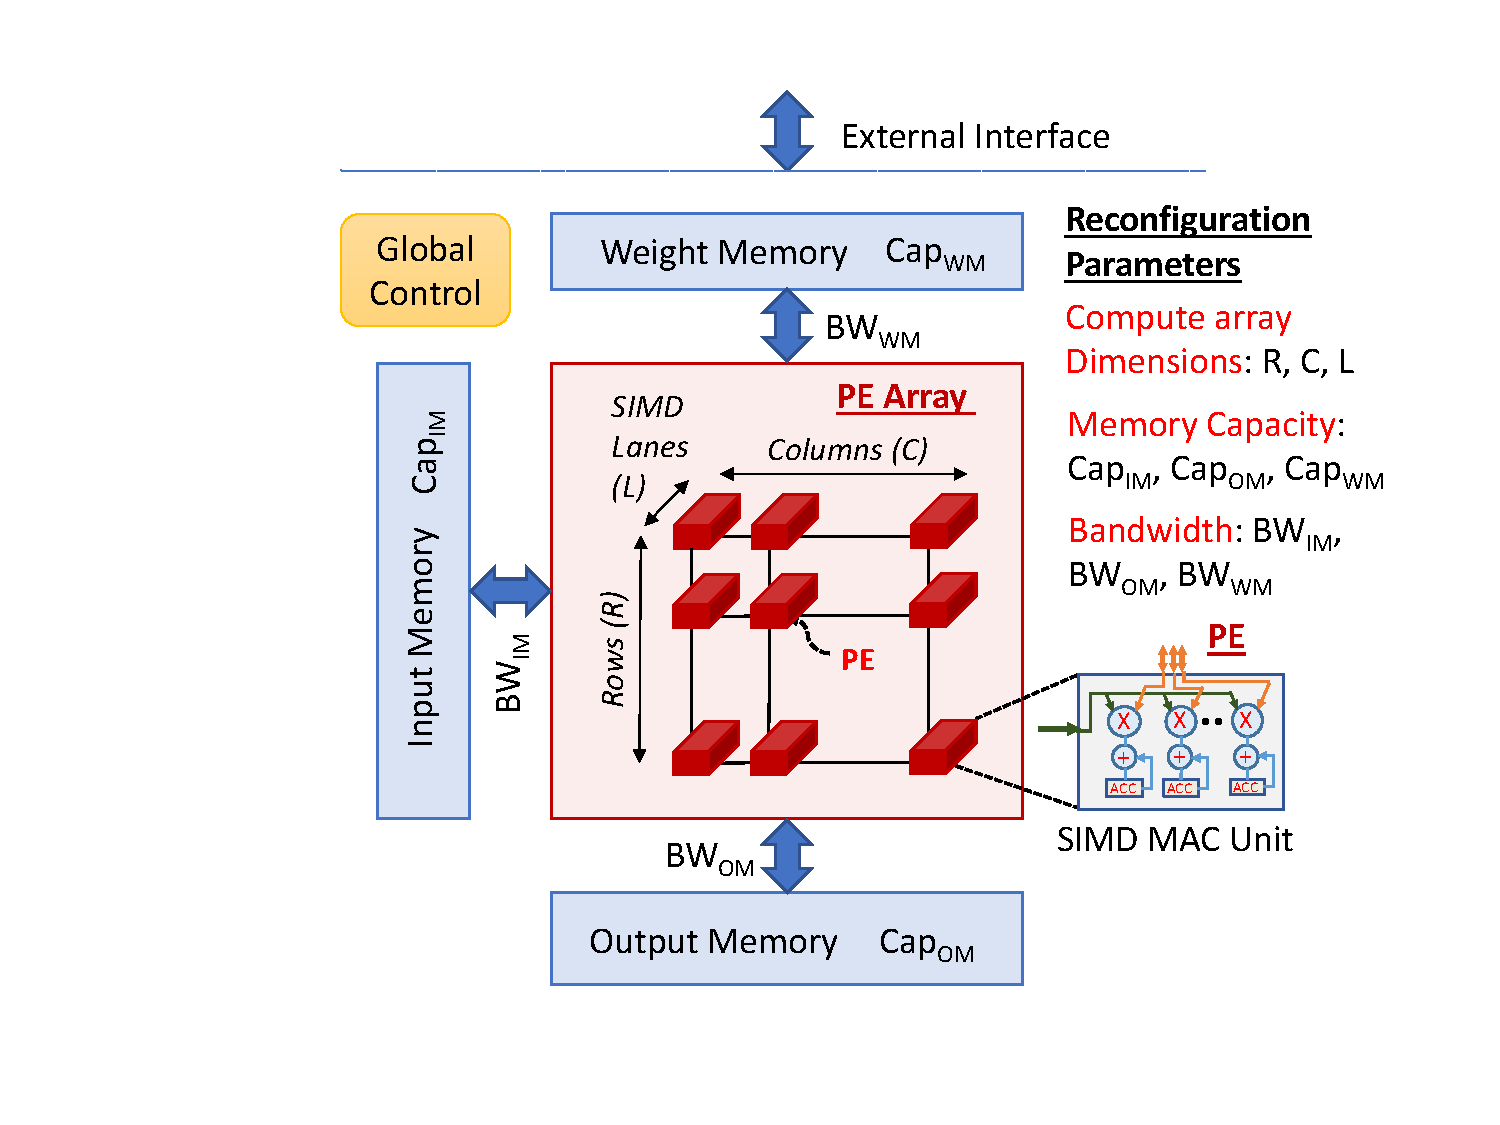
\includegraphics[width=0.5\linewidth]{figs/syst-array.pdf}
    \caption{A SIMD 2D systolic array accelerator}
    \label{fig:systolic_array}
\end{figure}

% \subsection{Enabling Dynamic Reconfiguration} \label{sec:enable-dyhard}

% \paragraphHeading{Embedded ASIC Implementation} 
% Figure~\ref{fig:reconfig-syst-array} shows an ASIC implementation of a 2D systolic array with reconfigurable enhancements.
% To redistribute compute, memory, and bandwidth resources, we add power and clock gating circuits to the rows and columns of the PE array, the memory banks, and the interconnect channels.
% Given a configuration map, the RCU enables the appropriate units at run-time.
% To vary the dimensions of the 2D array while keeping the number of PEs constant, we add \emph{fuse logic} between neighboring processing elements.
% For example to reduce the number of rows by half while increasing the number of processor lanes and columns, the fuse logic contains multiplexors to redirect the same input operand across both rows.
% The cost of reconfiguration is given by the time taken by the RCU to set the appropriate control registers in the design, which is feasibly completed in 10s of clock cycles.

% \paragraphHeading{Programmable SoCs with FPGA} 
% In the case of FPGA implementations, full or partial FPGA reconfiguration is used.
% Depending on the size of the bitstream, reconfiguration may take anywhere between hundreds of $\mu sec$ to a few $msec$.
% For example, loading a 94.4KB bitstream using an ICAP32 DMA onto a Xilinx Virtex5 FPGA takes $\sim324 \mu sec$~\cite{nafkha2016accurate}.
% Assuming a typical operating frequency of 100--200~MHz, reconfiguration may take anywhere between few hundred thousand to a million cycles.

% It is worth noting that the reconfiguration cost can be easily amortized by processing multiple inputs as a batch \ie, a layer is executed sequentially for several different inputs.
% This is naturally achieved in DNN training, as training inputs are batched.
% However, in our evaluation, we assume the worst case batch size of one.
% Also, we comprehensively sweep the range of reconfiguration overheads from ten cycles to a million cycles, and demonstrate benefits under all scenarios.

\subsection{Related Work}

Related work involves both accelerator optimization as well as quantization and compression.

\textbf{DNN Accelerators and Dataflow Optimization}
To improve the compute efficiency of DNN, a wide variety of accelerator architectures span the spectrum from low-power IP cores~\cite{du2015shidiannao,chen2017eyeriss,chakradhar2010dynamically,albericio2016cnvlutin,han2016eie,reagen2016minerva,eldridge2015towards} to large-scale systems~\cite{venkataramani2017scaledeep,jouppi2017datacenter,chen2014dadiannao}.
Almost all these efforts exploit the reuse pattern in convolutions and matrix-multiplications using a 2D-array of processing elements and an associated data-flow.
Some key architectural ideas proposed in these efforts include the use of heterogeneous processing cores for multiply-and-accumulate \emph{vs.} special-function operations, software-managed distributed memory hierarchy, on-chip and off-chip interconnect topologies that match the DNN's communication patterns, exploiting the sparsity in computations, among others.

Very few efforts have proposed optimizations considering the heterogeneity in compute characteristics across layers in DNNs.
For example, Eyeriss~\cite{chen2017eyeriss} modulates the dataflow in software between weight stationary \emph{vs.} row stationary depending on layer characteristics.
ScaleDeep~\cite{venkataramani2017scaledeep} builds two types of chips to realize CONV and FC layers respectively.
In contrast, for the first time, we propose to dynamically reconfigure hardware parameters, redistributing resources between compute, memory and bandwidth, determined by the layer's requirements.

\textbf{Quantization and Compression}
Techniques such as  reduced precision implementations~\cite{reagen2016minerva} and model compression~\cite{han2016eie} for improving an accelerator's efficiency by leveraging its error resilient nature have been extensively explored.
These efforts are complementary to \dyhardDnns, \ie, they can be applied on top of dynamically reconfigured hardware for further benefits.

\section{Task 2: Acceleration of Biological Neurons as Automata}

\subsection{Problem Definition}

Neuroplasticity in the brain allows it to learn and to recover cognitive ability following changes at levels ranging from individual neurons to entire cortices~\cite{wikipedia2018neuroplasticity}.
Hierarchical temporal memory (HTM) is a machine learning model that mimics biological neurons with high accuracy, designed to capture brain-like cognitive capabilities of the neocortex in software~\cite{hawkins2006hierarchical, hawkins2010hierarchical}.
HTM can autonomously learn to predict future states from a stream of temporal data, and has demonstrated aptitude in several prediction and anomaly detection applications~\cite{doremalen2008spoken, lavin2015evaluating, ahmad2016real, bonhoff2008using}.
Additionally, its biomimetic properties make it resilient to changes such as pruning neurons and synapses~\cite{mnatzaganian2017mathematical, ahmad2015properties}.

CPU-based simulators for spiking networks such as Compass~\cite{preissl2012compass} and SpiNNaker~\cite{painkras2013spinnaker} use von Neumann-based architecture, which is a fundamental bottleneck for large-scale, massively interconnected neural models.
Specialized neural network accelerator hardware, such as the IBM TrueNorth~\cite{merolla2014million} and the Qualcomm Zeroth~\cite{kumar2013introducing} platforms, employ concepts that are direct analogues from biology, and use spatial architecture to mitigate memory bottleneck issues.
Existing accelerators customized for HTM so far implement a quantity of cells not capable of supporting real-world sized applications~\cite{fan2016hierarchical}.

The Automata Processor (AP) is a silicon implementation of non-deterministic finite automata that can be programmed to recognize patterns in a stream of temporal data~\cite{dlugosch2014efficient}. 
Several natural correspondences between the execution model of the AP and of HTM suggest that an efficient mapping could capture significant speedups and desirable scalability due to its highly parallel execution model~\cite{putic2017hierarchical}.
Despite these correspondences, a key challenge of implementing HTM in the AP is that the lack of arithmetic capability of the AP means that it cannot natively support core HTM algorithms.
Furthermore, the costs of direct line on-chip communication modeling inter-cellular activations place an upper bound on the total number of cells that can be modeled, consequently limiting its real-world applicability.

The key idea of the proposed approach is to map the cell model of HTM to the AP to take advantage of the massive automata parallelism provided by its many parallel match elements to capture significant speedups over existing accelerators.
Instead of spending time coalescing data from sparsely distributed synapses before computing activations for each neuron as in the von Neumann model, the AP model receives a single, global data stream, and each cell computes its activation independently.
This approach essentially eliminates marginal cell bandwidth and scalably facilitates full-size models that can support useful, real-world HTM-based applications.

This approach is made possible by three key insights: (i) the resilience of the core dendritic segment activation algorithm can be exploited to \textit{approximate} it as a decision problem, allowing cells to be realized as independent, counter-enhanced automata (CEA) on the AP, eliminating the von Neumann bottleneck to capture speedups, (ii) inter-cellular communication can be separated into an off-chip phase, eliminating thread divergence, and allowing linear space complexity, and (iii) HTM's sparse connection properties can be leveraged to achieve average-case linear temporal scalability when synaptic connections are converted into temporally-spaced communications.

\subsection{Research Hypothesis}
In proposing this work, we hypothesize that \textit{if} changes are made to the core HTM algorithms to make it compatible with implementing it in the AP, \textit{then} despite the necessary approximations, applications using the resulting model will have significantly better throughput and more desirable resource scalability, while maintaining near constant application accuracy with the baseline.

% near-constant accuracy within a magnitude of the baseline CPU algorithm, will capture significant ($> 10$X) speedup, and will exhibit linear scalability.

\subsection{Contributions}
% Despite that the AP is a silicon implementation of nondeterministic finite automata, the process of translating the AP model from the baseline Python code requires a novel approach by considering the AP as a kind of specialized FPGA.
% To implement this approach, we will develop a general methodology and associated compiler software for the synthesis of trained HTM models as automata, which accepts trained HTM parameters and a set of hierarchical element templates as inputs to generate an AP-compatible model.

This research will make the following contributions:
\begin{itemize}
    \item To demonstrate functionality and to show how the AP can be used as a specialized FPGA, we will introduce a model of HTM neurons as CEA that exploits the correspondences between the HTM neural model, CEAs, and the AP spatial architecture.
    \item To facilitate the synthesis, simulation, and validation of general HTM models as CEA, we will develop a general methodology and associated software tools to map trained HTM models to the AP architecture, and dataflow tools for pre- and post-processing inputs and outputs.
    \item To validate the potential speedups and scalability benefits and to facilitate comparisons with related work, we will simulate several appropriate HTM benchmarks and develop resource scalability models.
\end{itemize}

To evaluate these ideas on the AP architecture, we will use Micron's ANML structural design language for the AP, and will use the AP toolchain that provides a software simulator.
Additionally, results will be validated using the VAsim~\cite{wadden2016vasim} toolchain.

\subsection{Motivating HTM Models As Automata}

In this section, we motivate the realization of HTM models as automata by highlighting key correspondences between HTM and AP execution models.

\subsubsection{Key Correspondences}

\textbf{Cell activation}
HTM cells and the AP's STE elements have similar state transition models.
When STEs are activated by other elements, they ``listen'' to the input stream, and report when a matching string is seen.
Similarly, HTM cells are enabled by external inputs through column dendrites and activate through lateral connections on local dendrites if they were predicted to do so by cells in a previous epoch.

\textbf{Streaming dataflow model}
Both STEs and HTM cells operate on continuous streams of data.
The AP natively implements regular expressions, which take strings of characters as input.
Matches can also internally activate other elements.
Similarly, in HTM, a stream of SDRs causes column activations, which activate cells whose lateral activations predict upcoming inputs.
In both memory paradigms, input sequences are matched against stored patterns, which both constitute outputs and laterally enable ensuing elements to listen to the input and continue processing.

\textbf{SDR bit overlap similarity}
Similarity between SDRs is determined by counting the number of overlapping bits.
An analogous operation in the AP can be implemented by using STEs with symbol sets programmed for active bit indices, attached to a counter that accumulates the number of overlapping bits as the SDR active bit indices are provided on the input.

\textbf{Model parallelism}
The AP can be programmed with a single automaton, or many independent, parallel automata, that all operate on the same input stream, and internally communicate state through activations.
Similarly, HTM columns and cells operate independently and communicate cell state laterally through synaptic connections.

\textbf{Hierarchy}
Connection among multiple APs is flexible, which can be configured to all receive the same input stream, or multiple independent streams.
Using intra-rank bussing, multiple APs could be configured to act as multiple HTM regions in a hierarchy.

\subsubsection{Counter-enhanced Automata HTMs Key Insights}

To motivate HTM models as counter-enhanced automata, we highlight design methods that leverage correspondences between the AP and HTM to convert HTMs into automata that are compatible with the AP's execution model.

\textbf{Dendritic segment activation as decision problem}
HTM column and cell state variables (i.e., active, predicted, bursting, etc.) are binary, and next-state values of these variables are computed using counting and simple Boolean functions.
STEs and counters can be used to store and count these variables, and the inherent Boolean properties of STEs can be used to implement next-state transition functions.
For example, automata states in the AP natively \texttt{OR} their inputs, and automata naturally implement the \texttt{AND} function by matching when a state is connected to the input and it receives a matching input.

\textbf{Virtual synaptic connections}
Implementing synapses with physical connections between STEs in the AP would not be scalable due to practical routing and fan-out limits.
Instead, to take advantage of the MISD organization of the AP, cells can be connected ``virtually'' between epochs via the input stream, taking advantage of the high-bandwidth on-chip broadcast network on the AP.

\begin{figure}
    \centering
    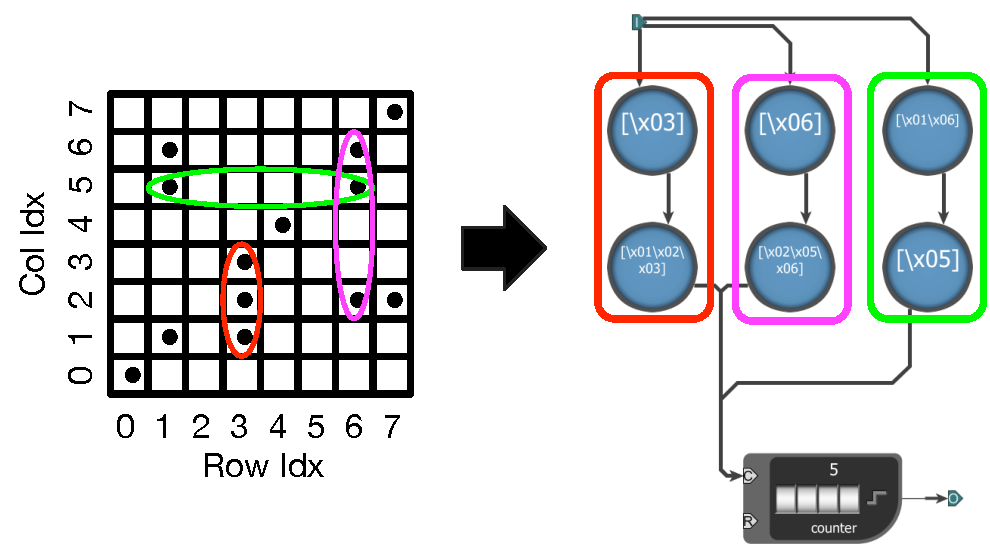
\includegraphics[width=0.5\linewidth]{figs/sparse_matrix_widget.pdf}
    \caption{Example of an AP segment automaton construction.
    Connections between cells can be expressed as a sparse matrix (left).
    This sparse matrix lookup table is implemented in the AP with parallel automata that are OR-ed together and counted (right).
    When active connections are scanned in on the input, the counter's threshold is crossed if a sufficient number of connected synapses are present.
    Using two 8-bit symbols on the input, this type of automaton can model connections from any number of up to 65,536 cells.\label{fig:sparse_matrix_widget}}
\end{figure}

\textbf{Dendrite segments as automata}
HTM cells activate if any of its dendrite segments received a sufficient number of active synapses, of which the threshold is determined as part of HTM learning.
The AP's counter element counts STE activations and reports if a threshold is crossed, and is a natural way of counting activations to determine if a cell was predicted.
The automata connected to the counter implement a sparse connection matrix, as shown in Figure~\ref{fig:sparse_matrix_widget}.
With unique $(row, col)$ IDs assigned to each cell, connections between the output of that cell and the segment are encoded in the symbol set of the STE elements.
The segment recognizes an activation from any other cell in the HTM.
The first STE matches on the $row$ ID, and the second matches on the $col$ ID.

To construct the automata in an efficient manner, we take advantage of the parallel lookup property of STEs, and use a method similar to Karnaugh maps.
For example, to represent connections from cells $((3, 1), (3, 2), (3, 3))$, the $row$ STE is programmed to recognize the symbol set $(3,)$ and the $col$ recognizes $(1, 2, 3)$.
It does not matter if the same $(row, col)$ ID is encoded in two different groups because counters \texttt{OR} their inputs and increment only once, regardless of the number of simultaneous activations.

The input data stream is then constructed of a string of $(row, col)$ IDs of cells that activated in the previous epoch.
At the end of the input tape, counters that crossed their thresholds mean a sufficient number of active connections were received, indicating the associated cell was predicted.

Although cells in HTM can potentially connect to any other cell in the region, due to the sparseness property, at most, this is about 2\% of the total number of cells, and in practice, it is far less. This ensures that the size of each segment in the AP is kept within reasonable bounds.

\textbf{Winner selection by thresholding}
Only those cells in columns with active segments from the input above a certain threshold are eligible to activate in the temporal memory phase.
Although similar to the temporal memory dendrite activation method, the HTM spatial pooler algorithm selects column activations based on a k-winners-take-all algorithm, which necessarily requires sorting.
Since sorting cannot be implemented efficiently on the AP, the global inhibition algorithm as part of the spatial pooler was modified to eliminate this dependency and to facilitate parallelization.
Although sometimes resulting in incorrect column activations, the resilience property of HTM ensures that good overall accuracy is preserved.

\begin{figure}
\centering
\begin{minipage}{.5\textwidth}
  \centering
  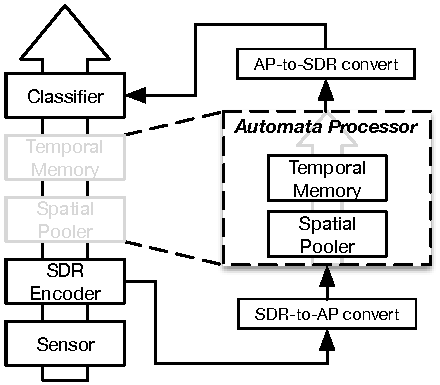
\includegraphics[width=.66\linewidth]{figs/HTM_AP_Architecture_Diagram.pdf}
  \captionof{figure}{Overview of the HTM stack with the SP and TM layers offloaded to the AP.}
  \label{fig:test1}
\end{minipage}%
\begin{minipage}{.5\textwidth}
  \centering
  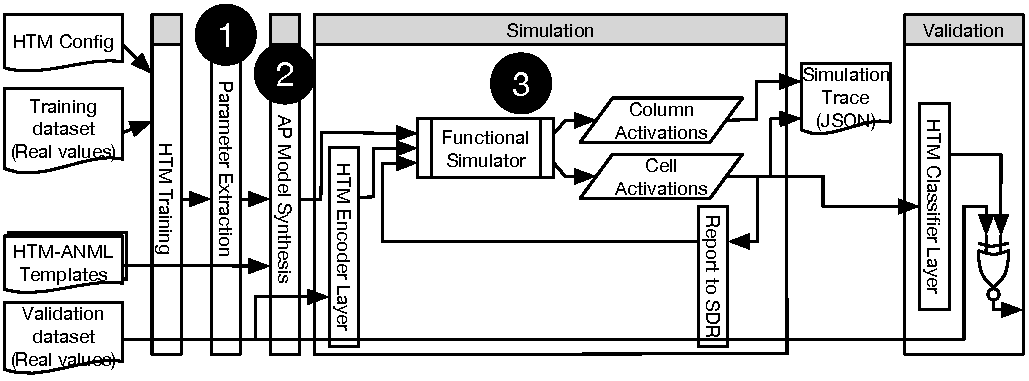
\includegraphics[width=\linewidth]{figs/HTM_AP_Workflow.pdf}
  \captionof{figure}{Overview of the Dendroplex components for synthesis, simulation, and validation of HTM models in the AP.}
  \label{fig:HTM_AP_Architecture_Diagram}
\end{minipage}
\end{figure}

\subsection{Proposed Approach}

Figure~\ref{fig:HTM_AP_Architecture_Diagram} shows an overview of the proposed approach.
Parameters from a trained HTM will be synthesized into a model suitable for simulation and compilation on the AP, in the ANML structural definition language.
The HTM stack will be modified to include the AP-based core HTM functions in the flow while surrounding pre- and post-processing layers will continue to reside on the host, and data translation layers will be added. 

The proposed project will consist of three parts:
\begin{itemize}
\item \textbf{HTM Parameter Extractor Tool} This tool will take a trained HTM network as an input and output a set of cell labels and edges between cells that define the structure of the the HTM.
\item \textbf{HTM-ANML Compiler Tool} This tool will take the extracted structural definition of the HTM and will construct an ANML model of the trained HTM that is suitable for simulation.
\item \textbf{Simulation and Validation Methodology} This set of tools will contain three tools: (i) for converting sparse distributed representation inputs for an HTM benchmark to an AP input tape, (ii) for converting sparse distributed representation inputs into real-valued outputs, and (iii) for feeding inputs to the AP model under simulation and for capturing outputs.
\end{itemize}

\subsection{Evaluation Criteria} 
% The performance of the design will be evaluated using suitable HTM benchmarks.
% The difference between the baseline HTM model and the AP-based HTM model will be characterized by comparing the application error of benchmark applications, the runtime, and the number of each hardware resources needed to synthesize each benchmark.
A performance improvement will be shown if the resulting HTM-AP model completes the same core algorithm functions, including overhead, in less theoretical cycles than the baseline CPU model, using suitable benchmarks.
Evaluation of the theoretical scalability of the model will determine the number of hardware resources that are necessary as a function of the number of synapses, dendrites, and cells in the HTM model.
Good scalability will be achieved if the resulting design is bottlenecked by the more abundant STE components, rather than the more limited counter or logic elements of the AP.

\subsection{Related Work}

Previous works have introduced accelerator architectures for HTM. 
Billaudelle and Ahmad~\cite{BillaudelleAhmad} port core HTM functions to a spiking neural network ASIC and verify that it meets basic HTM properties. 
Zyarah~\cite{FPGAThesis} demonstrates impressive speedups in an FPGA implementation using small (100 cols., 300 cells) HTMs against a MATLAB baseline implementation. 
An additional work by Deshpande~\cite{InspiredThesis} builds an FPGA-based implementation of principle component analysis inspired by HTM.

The major difference between related works and ours is that we will validate our model with HTMs of non-trivial size (up to 1804 columns, 44k cells), using real application benchmarks.
Additionally, we will evaluate the communication overheads and scalability of our approach as a function of the number of synapses, dendrite segments, and cells of the baseline HTM model.

\section{Task 3: Hardware Optimization Based On Workload Semantics} 

\subsection{Problem Definition}

DNNs are increasingly being used in mission-critical applications, such as autonomous vehicle control systems, banking, and medical diagnosis.
Consequently, robust system design in the presence of soft errors in DNN accelerator architectures is a concern for applications ranging from resource-constrainted embedded to large-scale cloud platforms.
Such faults originating from high energy particle strikes or voltage noise, can propagate to the application if their effects are latched, and can cause errors if they are not detected~\cite{blome2006cost}.
Of the components in a DNN accelerator, SRAM is especially susceptible, due to its greater sensitivity to process, voltage, and temperature variation than logic~\cite{mitra2005robust}.

Designers use a variety of soft error detection and correction techniques to mitigate the effects of faults in static memory~\cite{mitra2005robust}.
Since technology scaling has lowered the energy threshold needed to cause upsets, error correction codes (ECC) are becoming insufficient to mitigate the growth in such events in SRAM as process scaling has progressed~\cite{ganapathy2017characterizing}.
Selective precision scaling is also be used to improve resilience by allocating bit depth based on neuron criticality~\cite{venkataramani2014axnn, koster2017flexpoint}.
Circuit-level hardening and physical redundancy approaches come at the cost of significant area overhead, and the associated power costs and reduction in performance.
Replication techniques such as N-modular redundancy (NMR) and redundant multithreading (RMT) are classical approaches for soft error protection through replication of vulnerable operations, that come at the cost of additional latency, power, and area.
Comprehensive resilience methodologies, such as CLEAR can offer cross-layer resilience~\cite{cheng2017tolerating}, optimizing based on the best technique for each design layer.

Any number of these techniques can be applied to significantly improve the resilience characteristics of DNN accelerators.
However, a key limitation of doing so without knowledge of application-level characteristics is that soft error protection techniques are applied uniformly.
Consequently, significant power, area, or latency costs are incurred, reducing the efficiency of the hardware.

\textbf{Heterogeneous Neural Sensitivity}
In contrast, we observe two key insights: (i) that the contribution of the output among neurons to the accuracy of the application is non-uniform, and (ii) that non-critical neural operations provide a degree of fault masking for free, allowing savings by reducing or eliminating error protection where possible.
% The process of back propagation during training results in groups of neurons that are responsive to sets of features in the input that correlate to each output class.
Not all of the features in the input contribute the same amount to the accuracy of the output.
Consequently, the same error magnitude on the output of some neurons may contribute widely varying amounts to a change in the accuracy of the application, and is therefore more or less critical. 

\textbf{Selective Application of Soft Error Protection}
The key idea in our approach is to make more efficient use of myriad soft error protection techniques in DNN accelerators by determining the minimum necessary protection factor needed for each neuron according to its criticality.
Variation in sensitivity can be used to rank neural operations in order of criticality, and to selectively guide the application of soft error protection.
After this optimization, when transient faults occur, their effects on high criticality neurons are masked by the protection technique, while their effects on low criticality neurons are inherently masked by the application.
As a result, efficiency over uniform application is achieved by the significant reduction in circuit power, area, or latency while the overall application resilience benefits are preserved.
And since neural sensitivity is already determined during back propagation, the overhead of this step is natively built in to the DNN training process.

\subsection{Research Hypothesis}
In proposing this work, we hypothesize that \textit{if} soft error protection is applied to neural operations in a DNN accelerator according to their average criticality in the application, \textit{then} when the resulting DNN is executed using an appropriate validation dataset, resilience and accuracy characteristics of a comparable uniformly applied protection technique will be preserved, with improved hardware runtime metrics.

\subsection{Contributions}

\begin{itemize}
\item We characterize the resilience of several DNN applications in the presence of bit faults in a range of fault rates.
\item We propose a novel approach for exploiting the diversity in neural operation criticality to significantly improve the efficiency of soft error protection techniques in DNN accelerators.
\item We develop a resilience optimization methodology for determining the degree of soft error protection needed for each neuron to meet a set of design constraints.
\item We study the energy-resilience tradeoff space made possible by soft error protection techniques across a range of microarchitectural parameters that models embedded and cloud platforms, giving application designers opportunities to make tradeoffs between circuit-level metrics and application accuracy.
\end{itemize}

We will evaluate this methodology for real-world DNN applications using full validation datasets, and characterize the distribution of neural sensitivity for each.
To evaluate the costs and benefits of the methodology, we will use replication and majority voting as an implementation of soft error protection.

\subsection{Motivating Non-uniform DNN Redundancy}

In this section, we will motivate the need for applying non-uniform redundancy in the context of DNN applications for significantly improving the runtime metrics of spatial array DNN accelerators.

\subsubsection{Neural Network Training Background}

During the training process, the weights of neurons are adjusted so that the output of the network matches the expected output, and in so doing, it is iteratively trained to maximize accuracy.
Training consists of two steps: (i) inference and (ii) backpropagation.
During \textit{inference}, or forward propagation, an input is provided to the network and the output is calculated by propagating linear combinations of the inputs and weights forward through a sequence of layers in the network until the final output is calculated.
The error is then calculated between the predicted output and the expected output of the network.
During \textit{backpropagation}, the contribution to the output error of every neural input is calculated so that the weights can be adjusted to minimize the error.
Equation~\ref{eqn:backprop} as part of backpropagation, provides a method to compute a neuron's weight error ($\partial w$), and to relate the contribution of that error to the final output error ($\partial C$), based on the output of the neuron ($a$), and the error at the output of the neuron ($\delta$)~\cite{nielsen2015neural}.

\begin{equation}
\frac{\partial C}{\partial w_{jk}^{l}}=a_{k}^{l-1}\delta_{j}^{l}
\label{eqn:backprop}
\end{equation}

\subsubsection{Non-uniformity in DNN neuron criticality}

Non-uniformity of the criticality of neurons is granted by the expectation of non-uniform spatial locality present in a real dataset.
For example, if a neuron is connected to a region of input that rarely contains any features, its output will have a lesser impact on the final output, than one that often sees important features.
The weight of the neuron determines how much of its input it will pass to the output, and ultimately to the final output.
The process of training adjusts weights on neurons such that those connected to parts of the input with features that correlate highly to the correct output contribute more strongly to the output.
Therefore, we intuitively expect that neurons with more error in their weights are those that contribute non-critical information, and \textit{vice versa}.

% Warrants further investigtaion of the distribution of criticality among layers; criticality within a layer is not understood,

\subsubsection{Disadvantages of uniformly applied error protection techniques}

Existing soft error techniques applied uniformly leave unnecessary design margin for neurons that do not need the added protection.
Non-critical neurons receiving the same amount of protection as critical neurons leaves unclaimed design margin.
For example, although a fault in the weight value of a non-critical neuron may produce an error on its output, its output value will not be weighed as heavily on the path to the final output.
Such a neuron does not need protection.
A neuron that has low weight error means that the network considers its output important to the final output, and an error in the output of such a neuron would contribute a large error to the final output.
% For this reason, this neuron needs protection against soft errors that could negatively impact 

\subsubsection{Selective soft error protection}

Using neuron sensitivity as a proxy for resilience to direct the application of soft error protection, soft error protection is then applied to neurons proportional to their criticality.
For example, using replication as a protection technique, neurons requiring the highest protection would be classified into categories requiring none, three, or four times replication.
As a result, savings at the circuit level are claimed by using less power, area, or completing operations in less time, while maintaining accuracy at an equivalent fault rate.

\begin{figure*}
    \centering
    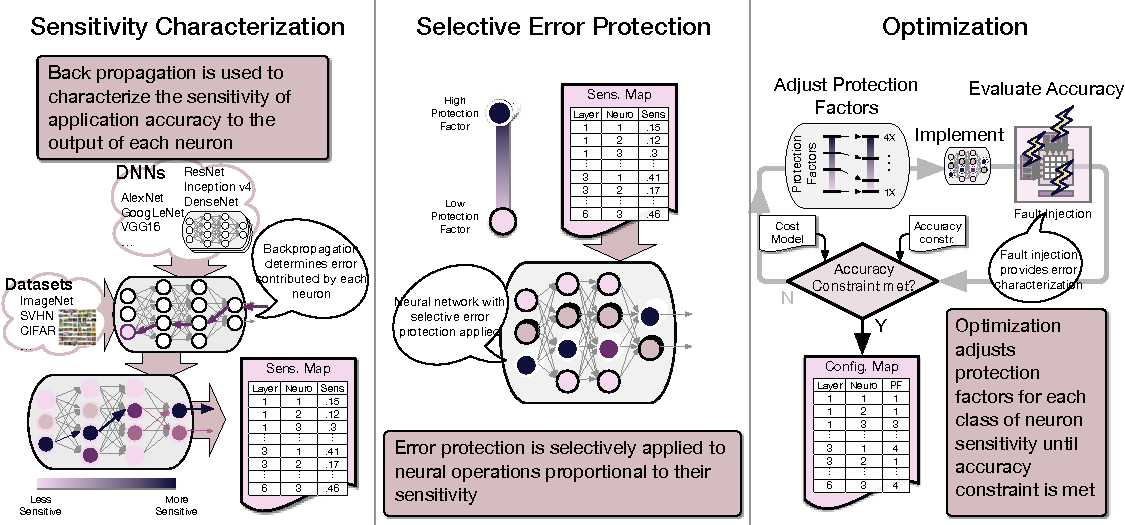
\includegraphics[width=\linewidth]{figs/DoggettOverview.pdf}
    \caption{Overview of Doggett methodology}
    \label{fig:fault_injection_overview}
\end{figure*}

\subsection{Proposed Approach}

Figure~\ref{fig:fault_injection_overview} shows an overview of the proposed approach for characterization and optimization of selective application of soft error protection for resilient DNN accelerators.

\subsubsection{Sensitivity Characterization}

To conduct sensitivity characterization, using a method similar to that outlined in~\cite{venkataramani2014axnn}, for each example in the training set, we can collect the error of the weights and biases of each neuron to compute the average error contributed over the entire dataset.
The resulting average error contribution can then be used as a proxy for the sensitivity of the output accuracy to each respective neuron, and can be used as a key to sort and classify the neurons into a sensitivity map.
% In the context of soft errors, non-uniform criticality means that in the average case, the effect of a single-event upset that changes the value of the output of a neuron on the output of the total network is not equivalent across all neurons.

\subsubsection{Selective Error Protection}

The purpose of the selective error protection phase is to calculate resource usage based on the initial classification of neurons into protection factors.
As part of the initialization step, each soft error protection technique defines its own cost of implementation.
For example, a precision-scaling technique would require hardware overhead for larger registers.
In the case of redundant multithreading, increased protection is achieved through multiple execution of a neural operation in time, followed by a majority voter, incurring a latency cost associated with repeated execution.

\subsubsection{Optimization}

Then during the optimization phase, given an accuracy requirement, a fault rate upper bound, and a fault protection cost model, the tool performs fault injection to evaluate the effects, and systematically minimizes the amount of protection needed for each neuron.
This process is repeated until the either the accuracy and resource constraints are met, or a solution cannot be found.
The output of this tool provides a mapping from each neuron in a DNN to the degree of protection that must be applied to it to meet design constraints.

Within this study, we will develop the following components:

\begin{itemize}
\item \textbf{Evaluation of the Effect of Bit Faults on DNNs} Several popular DNN workloads will be evaluated with full validation sets to evaluate the effects of faults on their accuracy and performance
\item \textbf{Resilience Optimization Methodology} The optimization methodology will consist of a mapping from neuron criticality to protection factors.
A further optimization step will determine how much protection factor to be applied to each neuron to meet accuracy and resource constraints.
\item \textbf{Resilience Optimization Tool}
The optimization tool will construct a sensitivity map from the analysis of criticality of neuron operations in the DNN.
These will be used to generate a set of configurations while considering total physical design constraints and the cost of soft error protection on an example circuit substrate.
This tool will also facilitate evaluation of the performance, power, and accuracy of a given soft error protection configuration map.
\end{itemize}

This methodology can be used to study and mitigate the effects of faults originating from one or multiple sources, each with a unique fault distribution. Furthermore, an extension of this work could be used to prioritize the fault resilience and associated hardware metrics of output classes, depending on their importance to the application.

% To address this question, we highlight two key insights: (i) the backpropagation and associated optimization phases are inherently flexible and can be used to minimize a loss function constructed to include circuit parameters, and (ii) in a trained network, there is significant variance among the impact that the output of a single neuron has on the final output function.
% Specifically, we propose that the first property can be used for low power design, and the second can be used to improve reliability without significant power and cost increase.

% For this piece, we will consider how resilience properties of DNNs can be exploited to either significantly save circuit power or to improve circuit resilience in DNN accelerators.
% To improve circuit-level resilience characteristics for spatial architecture accelerators, we propose to systematically explore resilient characteristics of DNNs to develop a methodology for making efficient energy-quality or resilience-quality tradeoffs at the architecture, logic, and circuit design levels.
% Both of these directions rely on the key observation that operations associated with low priority neurons can be either eliminated or run at reduced precision, enabling power reduction or performance increase via energy-quality tradeoff.

% To optimize the efficiency of accelerators, we try to reduce redundancy in the data by making it more sparse.
% While this makes the implementation more efficient, it also makes it more vulnerable to failures.
% For example, data types are chosen to provide just enough dynamic range and precision needed to meet application semantics~\cite{li2017understanding}, to reduce memory and communication requirements.
% However, when using common datatypes, which are dense, one bit represents a larger portion of the dynamic range, thus increasing its vulnerability.
% The challenge is to improve the resilience of DNN accelerators while maintaining good efficiency.

% The broad impact of the proposed work is that DNN accelerator hardware designers will have a systematic methodology to make tradeoffs between low power, resilience, and application output quality.
% The benefits of the proposed energy-quality tradeoff approach are captured in two ways: (i) in an \textit{iso-latency} regime, the technique results in an aggressive reduction of energy per computation, or (ii) in an \textit{iso-power} regime, performance is improved, with a small impact on output quality in both cases.

% This work is significantly different from previous approaches in two ways: (i) no previous approach has considered exploiting DNN resilience to enable voltage scaling.
% This approach is especially valuable because it exploits the quadratic relationship between supply voltage and power to yield much greater power savings than those that reduce area or runtime, while making relatively small impacts on quality.
% Furthermore, yield can be improved by making use of dies that did not meet baseline timing standards, but could still operate with reduced quality. 

% To enable significantly longer service lifetimes in systems with severely limited resources, we recognize that the length of logic paths can be normalized and the resilience properties of neural network application can be leveraged to enable controlled degradation of output quality.
% We will propose a project to evaluate the effects of voltage scaling on energy efficiency and application fidelity across a suite of suitable benchmarks.

\subsection{Evaluation Criteria}

Success in this project will be determined if The application accuracy will be within 10\% of the baseline, while the runtime characteristics (\ie, power, latency) will be measurably better than if the same soft error protection technique had been applied uniformly across all neurons, as determined by simulation.

\subsection{Related Work}

\textbf{Approximate Circuits}
Several previous works have proposed circuit reduction through precision scaling~\cite{venkataramani2013quality}, logic reduction~\cite{gupta2011impact, chippa2014storm, esmaeilzadeh2012neural}, approximating functions of less critical neurons~\cite{zhang2015approxann, venkataramani2014axnn, moons2016energy}, and caching or elimination of redundant operations~\cite{yasoubi2017power, han2015learning, misailovic2014chisel}.
The optimizations proposed in these works capture linear power savings by relying on either area reduction made possible by reducing the size of logic or number of gates needed to implement approximable functions, or runtime reduction by reducing the number of needed operations.

\textbf{Exploiting DNN resilience to improve circuit performance and power} Several papers~\cite{moons2016energy, kung2015power, moons2017dvafs} in this area introduce techniques for precision optimization as a means of saving power.
As an example, Venkataramani et al.~\cite{venkataramani2014axnn} introduce a methodology for making approximate the outputs of neurons with low impact on the output, and mapping these operations to corresponding approximate hardware to save power and improve performance.
Furthermore, they observe that retraining can be used to recover some of the quality impact of neuron approximation.
This work is significantly different from our proposed approach because it exploits datapath width scaling as a means of improving circuit metrics, whereas our proposed approach uses deliberate timing violation and voltage scaling.
As a result, our approach can achieve quadratic voltage scaling instead of linear.

Jiao et al.~\cite{jiao2017assessment} develop a method for optimizing the output quality of DNNs in the presence of errors caused by circuit-level process, voltage, and temperature variations.
They develop methods for simulating these effects by characterizing timing errors in an arithmetic circuit model and evaluating neural network performance in the presence of those errors.
While the error characterization approach is similar from the proposed approach, this work is different because it does not consider ways to improve circuit performance and instead focuses on application metrics.

% ~\cite{zhang2015approxann}

Zhang et al.~\cite{zhang2017enabling} uses a Razor\cite{ernst2003razor}-like timing speculation-based approach to detect and recover errors in MAC operations by inserting bubbles in the systolic array pipeline.
This work differs from our approach in that it does not consider restricting the set of values used in the network to those that cause short propagation delays.
Furthermore, it proposes delay penalties as a means of recovering errors instead of exploiting the resilience of DNN training.

Li et al.~\cite{li2017understanding} analyze software techniques for improving the resilience of DNN accelerators.
The main technique for improving the resilience of DNN accelerators introduced in this work is to harden latches following a bit-level sensitivity analysis.
While it serves to identify the effects faults on errors in DNN applications, it is sufficiently different in that it does not recognize the correspondence between the vulnerability of neurons within DNNs and the vulnerability of hardware components.

\newpage
\appendix
\section{Summary of Tasks and Deliverables}

\subsection{Task 1: Hardware Optimization Based on Workload Characteristics}

\begin{enumerate}
    \item \textsc{COMPLETE}: Develop a methodology for the optimization of neural network accelerators based on its dynamic workload characteristics, and evaluation with suitable DNN workloads
    \item \textsc{COMPLETE}: Design and implement a tool for optimization of spatial architecture hardware parameters based on the workload characteristics of DNN workloads
    \item \textsc{COMPLETE}: Evaluate energy-delay and efficiency tradeoffs of DNN workloads across several spatial architecture variants
\end{enumerate}

\subsubsection{Deliverables}

\begin{enumerate}
    \item \textsc{COMPLETE}: Publish results in first-author conference or journal publication (DAC, 2018)
    \item Open source release of codebase published to GitHub, with documentation
\end{enumerate}

\subsection{Task 2: Acceleration of Biological Neurons as Counter-Enhanced Automata}

\begin{enumerate}
    \item \textsc{COMPLETE}: Develop a functional model and methodology for synthesis of general HTM function in the identified spatial architecture
    \item \textsc{COMPLETE}: Apply the methodology to implement HTM in the chosen architecture, and evaluate performance and scalability in comparison to von Neumann architectures using suitable benchmarks
    \item \textsc{COMPLETE}: Design and implement a tool for the synthesis, simulation, and verification of general HTM models in AP architecture
\end{enumerate}

\subsubsection{Deliverables}
\begin{itemize}
    \item \textsc{COMPLETE}: Publish results in first-author conference or journal publication (IEEE MICRO, 2017)
    \item Open source release of codebase published to GitHub, with documentation
\end{itemize}

\subsection{Task 3: Hardware Optimization Based On Workload Semantics}

\begin{enumerate}
    \item Develop an approach for characterization of neurons by criticality
    \item Develop a methodology for determining the level of redundancy needed to achieve DNN application in the presence of faults
    \item Design and implement a tool for optimization of DNN redundancy based on the criticality of DNN neurons
\end{enumerate}

\subsubsection{Deliverables}
\begin{itemize}
    \item Publish results in first-author conference or journal publication
    \item Open source release of codebase published to GitHub, with documentation
\end{itemize}

\noindent
\subsection{Dissertation Chapters}
The expected main chapters of my dissertation are:

\begin{itemize}
    \item Optimization of runtime characteristics with dynamic hardware reconfiguration
    \item Mapping Hierarchical Temporal Memory to the Automata processor
    \item Optimization of soft error protection techniques with DNN resilience
\end{itemize}
\newpage

% \section{Preliminaries}

% DNNs are composed of compute units called \emph{neurons}, which are organized as a sequence of layers.
% Each layer is associated with a set of \emph{weight} parameters, which are combined with that neuron's inputs to determine its output.
% DNNs operate in two phases:
% In inference (i), when a new input is presented to the DNN, neurons in each layer are sequentially evaluated to produce a vector of outputs at the final layer.
% The input is classified to the class label corresponding to the neuron with the maximum output.
% In training (ii), weights associated with the layers are iteratively learned from a training dataset.
% In this case, the DNN is evaluated in both forward and backward directions, and the weights are updated after a \emph{batch} of training inputs.
% Although the concept of spatial architecture optimization is applicable both in the context of inference and training, in the proposed work, we illustrate the benefits for inference, which is performed several orders of magnitude more times than training.

% Artificial neural networks (ANNs)~\cite{mcculloch1943logical, hebb2005organization, farley1954simulation, rochester1956tests} are a broad class of machine learning algorithms that are inspired by both the structure and the functionality of biological neural networks, and are the basis of the majority of modern machine learning software applications.
% Broadly, neural networks are valuable because they do not require explicit programming, and can learn to form internal representations of datasets without 
% Neural networks come in many flavors, depending on the kind of data they process and the kind of output that is required.

% ANNs are operated in two phases: during \textit{training}, the functionality of the network is iteratively improved through exposure to input data as the internal weights are updated to match known good outputs.
% Then during \textit{inference}, the network is presented with a new set of inputs, the input data values are combined with the trained neuron weights in each layer in sequence until a vector of outputs is produced at the final layer.

% Classical neural networks, such as multilayer perceptrons (MLPs)~\cite{rosenblatt1961principles}, and more recently, convolutional neural networks (CNNs)~\cite{lecun1999object} are especially adept at autonomously extracting features and interpreting \textit{structural} data, such as images or other multidimensional signals.
% Deep neural networks (DNNs), modeled after the brain's visual and auditory cortices, contain many tens or hundreds of ANN layers~\cite{lee2009convolutional, simonyan2014very, sermanet2013overfeat, szegedy2015going, krizhevsky2012imagenet}, and have been used extensively and successfully for many applications focused on this type of data.

% In contrast, a related class of ANNs, called recurrent neural networks (RNNs), are designed to perform inference on \textit{temporal} signals.
% RNNs contain local storage and cyclical connections that combine elements of past inputs with current inputs to predict future inputs.
% As an example, hierarchical temporal memory (HTM)~\cite{ahmad2015properties, mnatzaganian2017mathematical} is closely modeled after the neocortex, and can learn to predict future outputs and detect anomalies by exposure to a stream of incoming data.
% A more mainstream RNN example is long-short term memory (LSTM), which is the main algorithm behind applications such as natural language processing and machine translation.

% \subsubsection{Characterizing Neural Network Workloads}

% \textit{Structurally}, ANNs are modeled as interconnected computational units called neurons, which are collected into a cascade of layers.
% Neurons accept a vector of inputs that are combined with internal weight parameters to produce an output, which is passed on to the next layer of neurons, and so on, the result of which is communicated to higher levels within a software framework.
% \textit{Functionally}, they can be trained to provide classification, detection, or prediction functions for various data types, while automatically generalizing from past experience.


\bibliographystyle{plain}
\bibliography{references,krycek-citations}
\end{document}
